\documentclass{beamer}
\usepackage{graphicx}
\usepackage{tikz}
\usepackage{float}
\usepackage{color}
\usepackage{multicol}

\usetheme{Copenhagen}
\usecolortheme{crane}

%Information to be included in the title page:
\title[Synchronized Chaos]{Sending Secret Messages with Synchronized
Chaotic Systems}
\author{Kevin Phan}
\institute{Harvey Mudd College}
\date{April 26, 2023}

\begin{document}

\frame{\titlepage}

\begin{frame}{Problem}
    \begin{figure}[H]
        
\includegraphics[width=8cm]{drawing.png}
        \centering
    \end{figure}
    \begin{itemize}
        \item Transmitter want to send a message $m(t)$ to Receiver. 
        \item Don't want anyone, but the receiver to be able to read the message.
    \end{itemize}
\end{frame}

\begin{frame}{Synchronized Chaotic System}
    \begin{columns}
        \begin{column}{0.5\textwidth}
           \begin{center}
            Transmitter 
           \end{center} 
           \begin{align*}
                \dot{x_T} &= \sigma (y_T - x_T) \\
                \dot{y_T} &= \rho x_T - y_T - 20x_T z_T \\
                \dot{z_T} &= 5x_T y_T - \beta z_T 
           \end{align*}
        \end{column}
        \begin{column}{0.5\textwidth}  
            \begin{center}
                Receiver 
            \end{center} 
            \begin{align*}
                \dot{x_R} &= \sigma (y_R - x_R) \\
                \dot{y_R} &= \rho x_T - y_R - 20x_T z_R \\
                \dot{z_R} &= 5x_T y_R - \beta z_R
            \end{align*}
        \end{column}
        \end{columns} 
         \bigskip
        \begin{itemize}
            \item Based on the Lorenz system. 
            \item The ``error'' decreases exponentially. 
        \end{itemize}
\end{frame}

\begin{frame}{Example of Synchronization}
    \begin{figure}[H]
        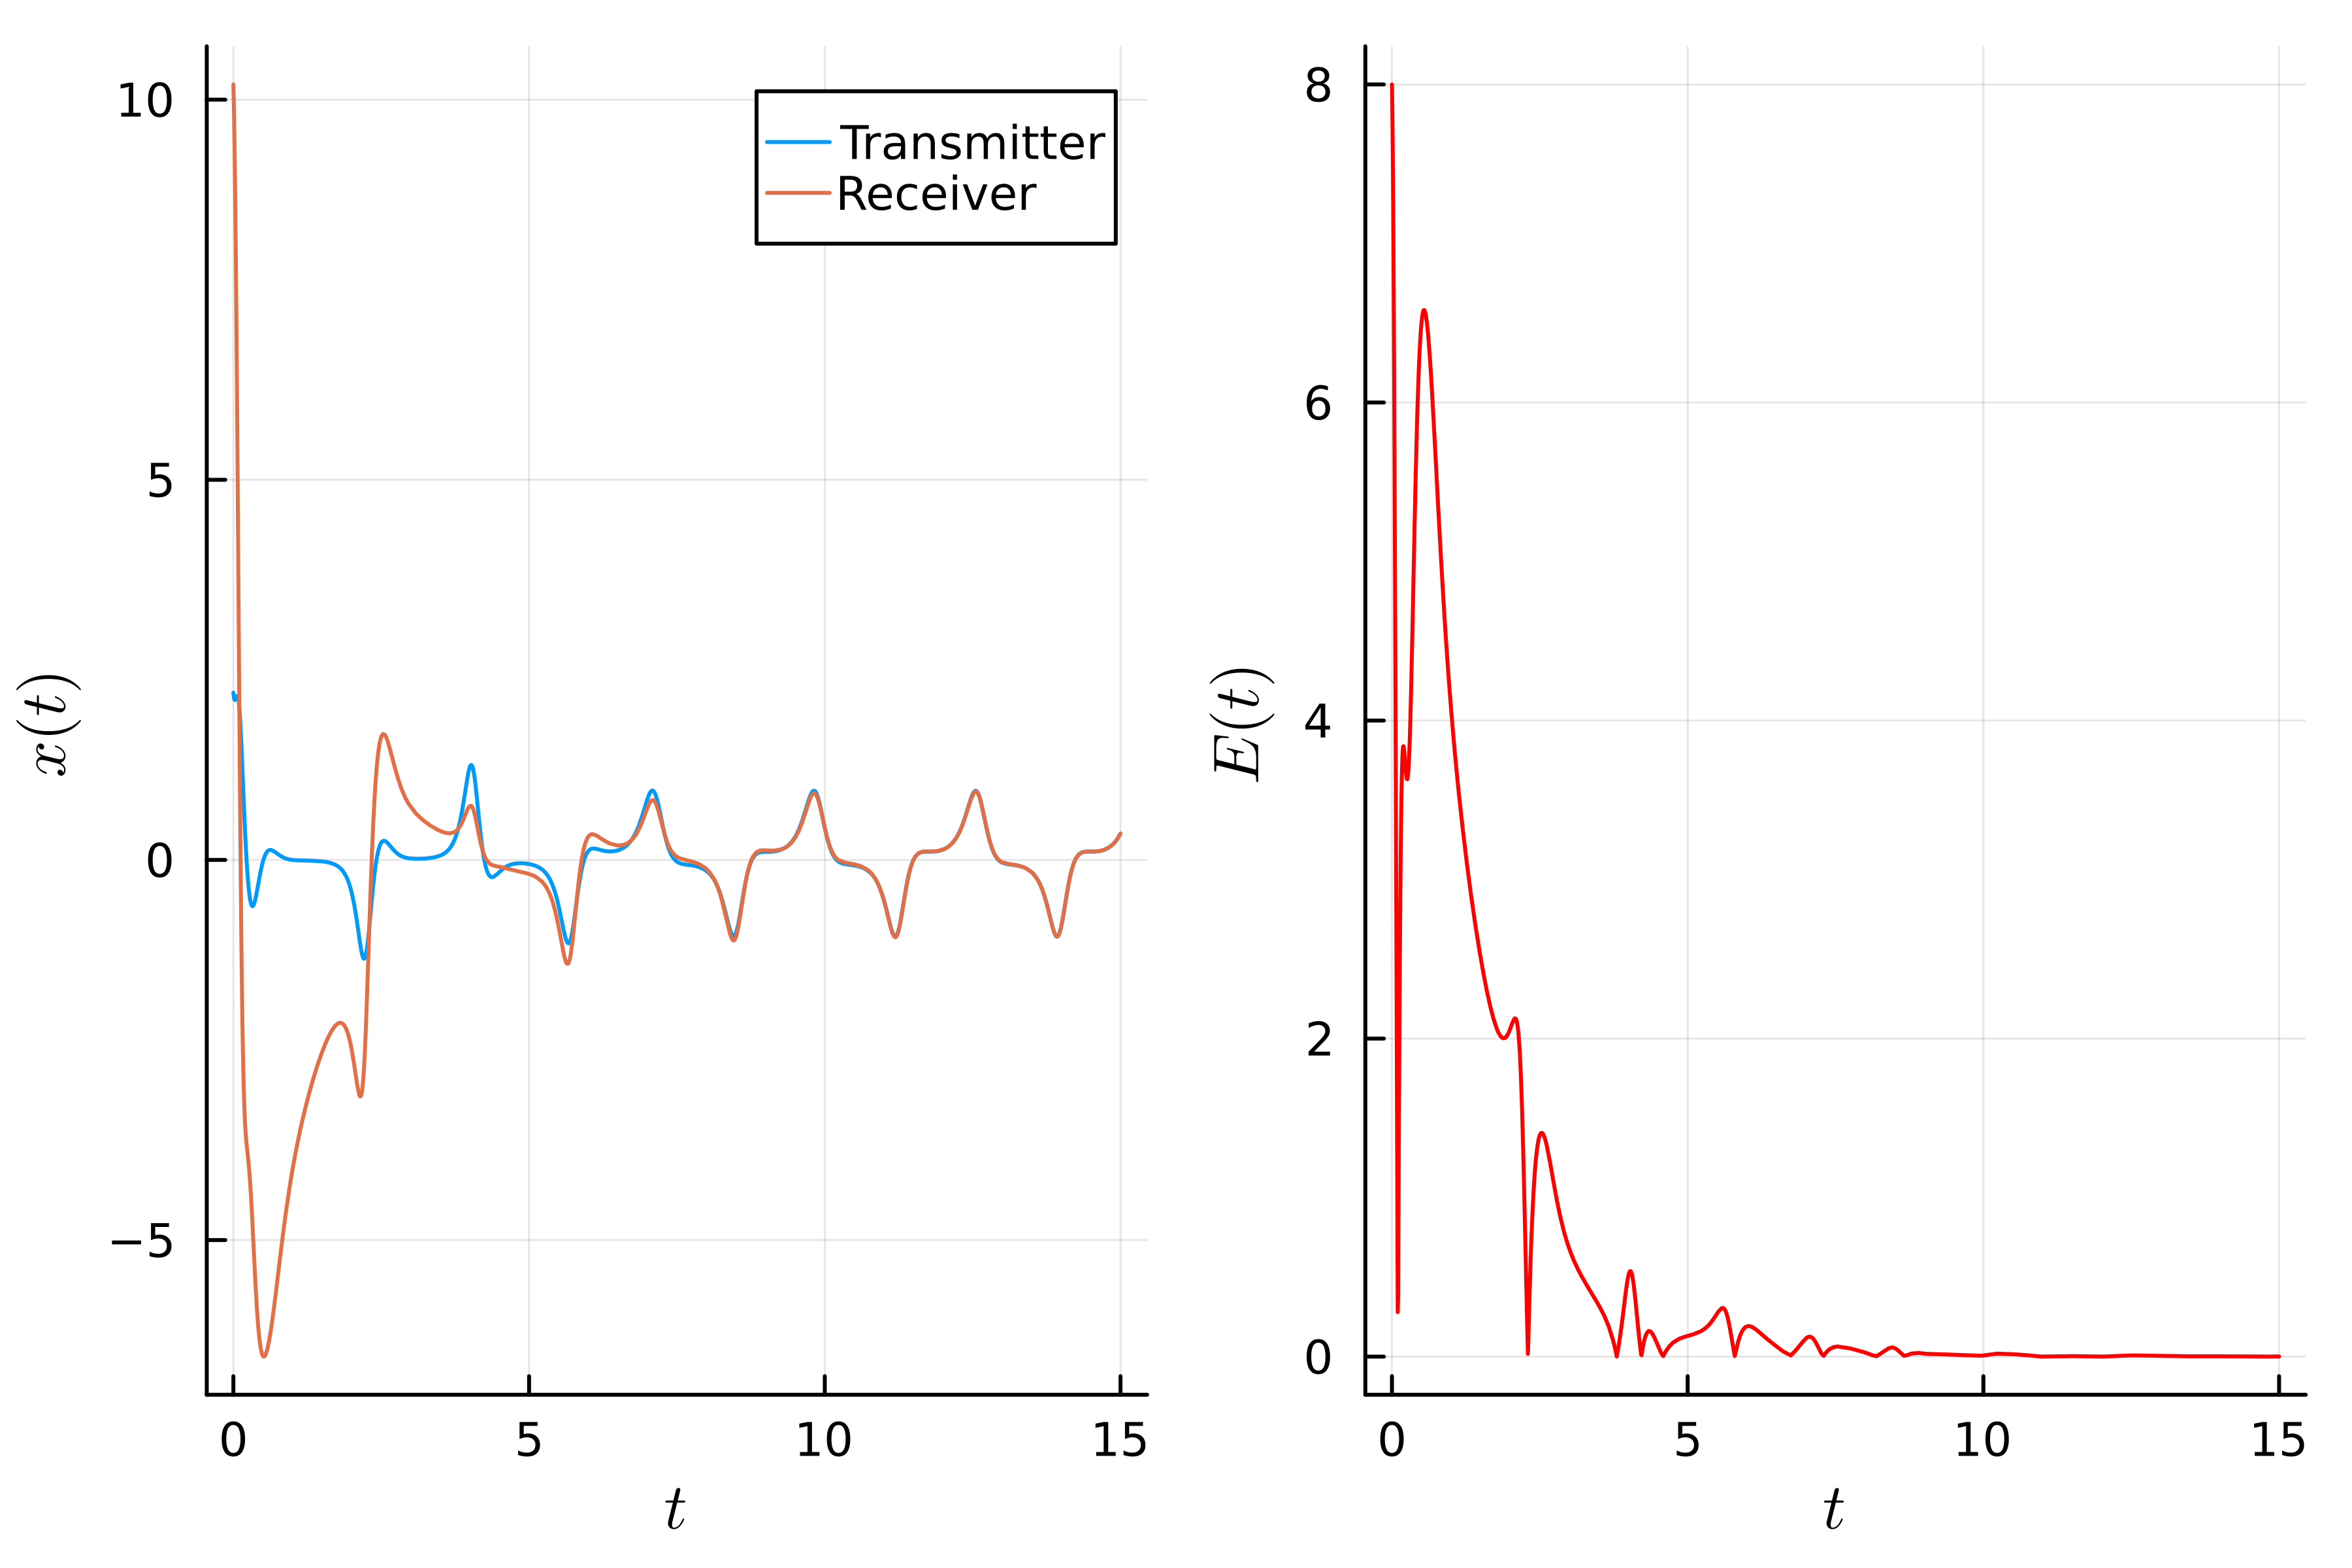
\includegraphics[width=\linewidth,height=\textheight,keepaspectratio]{combined_plot.png}
        \centering
    \end{figure}
\end{frame}


\begin{frame}{Algorithm to Send Secret Message}
    \begin{enumerate}
        \item Create encrypted message $\widetilde{m}(t) = x_T (t) + m(t)$ where $||m(t)|| \ll ||x_T(t)||$. 
        \item Send $\widetilde{m}(t)$ to the receiver. 
        \item Use the receiver's dynamical system which hopefully reproduce $x_R(t) \approx x_T(t)$. 
        \item Compute $\widetilde{m}(t) - x_R(t) \approx x_T (t) + m(t) - x_T(t) = m(t)$. 
    \end{enumerate}
\end{frame}

\begin{frame}{How Good is It?}
    \begin{figure}[H]
        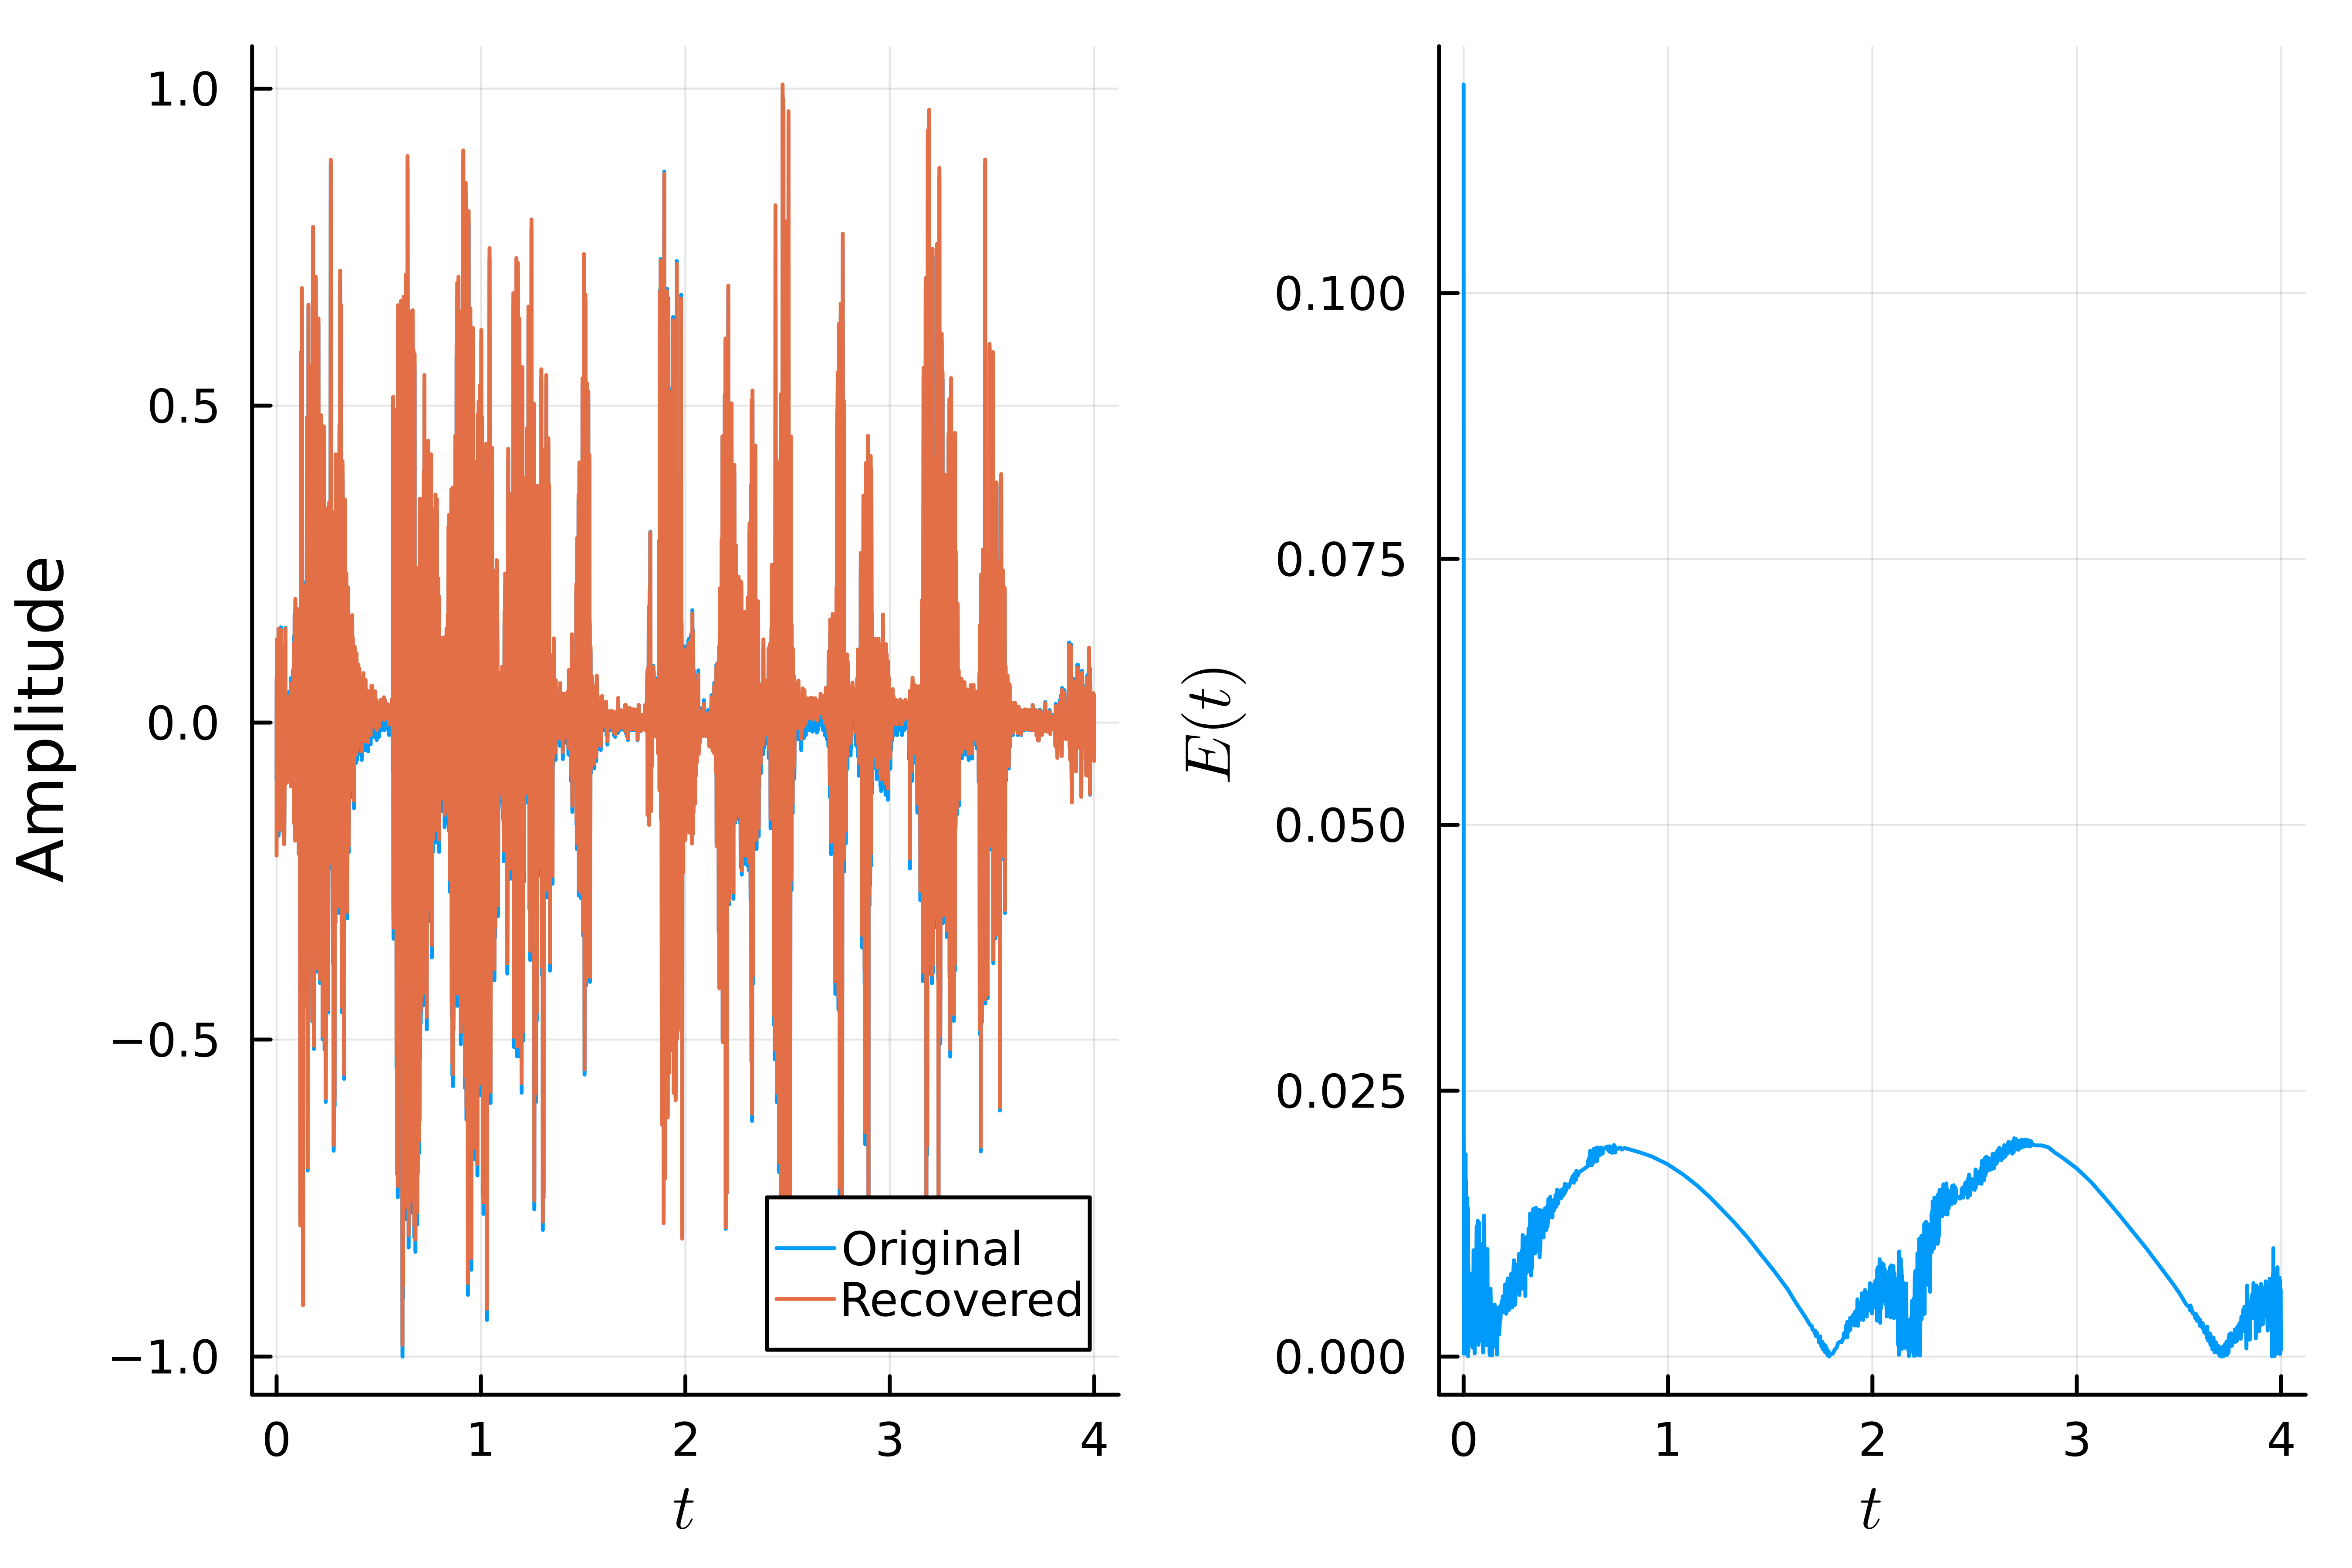
\includegraphics[width=\linewidth,height=\textheight,keepaspectratio]{combined_error_sound_plot.png}
        \centering
    \end{figure}
\end{frame}








\end{document}